\section{Supplementary results}
\subsection{Deep and periventricular WMH}
Here we present, in analogy to \Cref{fig:mv}, the results of the multiverse analyses of the association between cSVD burden, FO of DMN-related states, and executive function, when cSVD is operationalized as the volume of deep or periventricular white matter hyperintensities, respectively.

    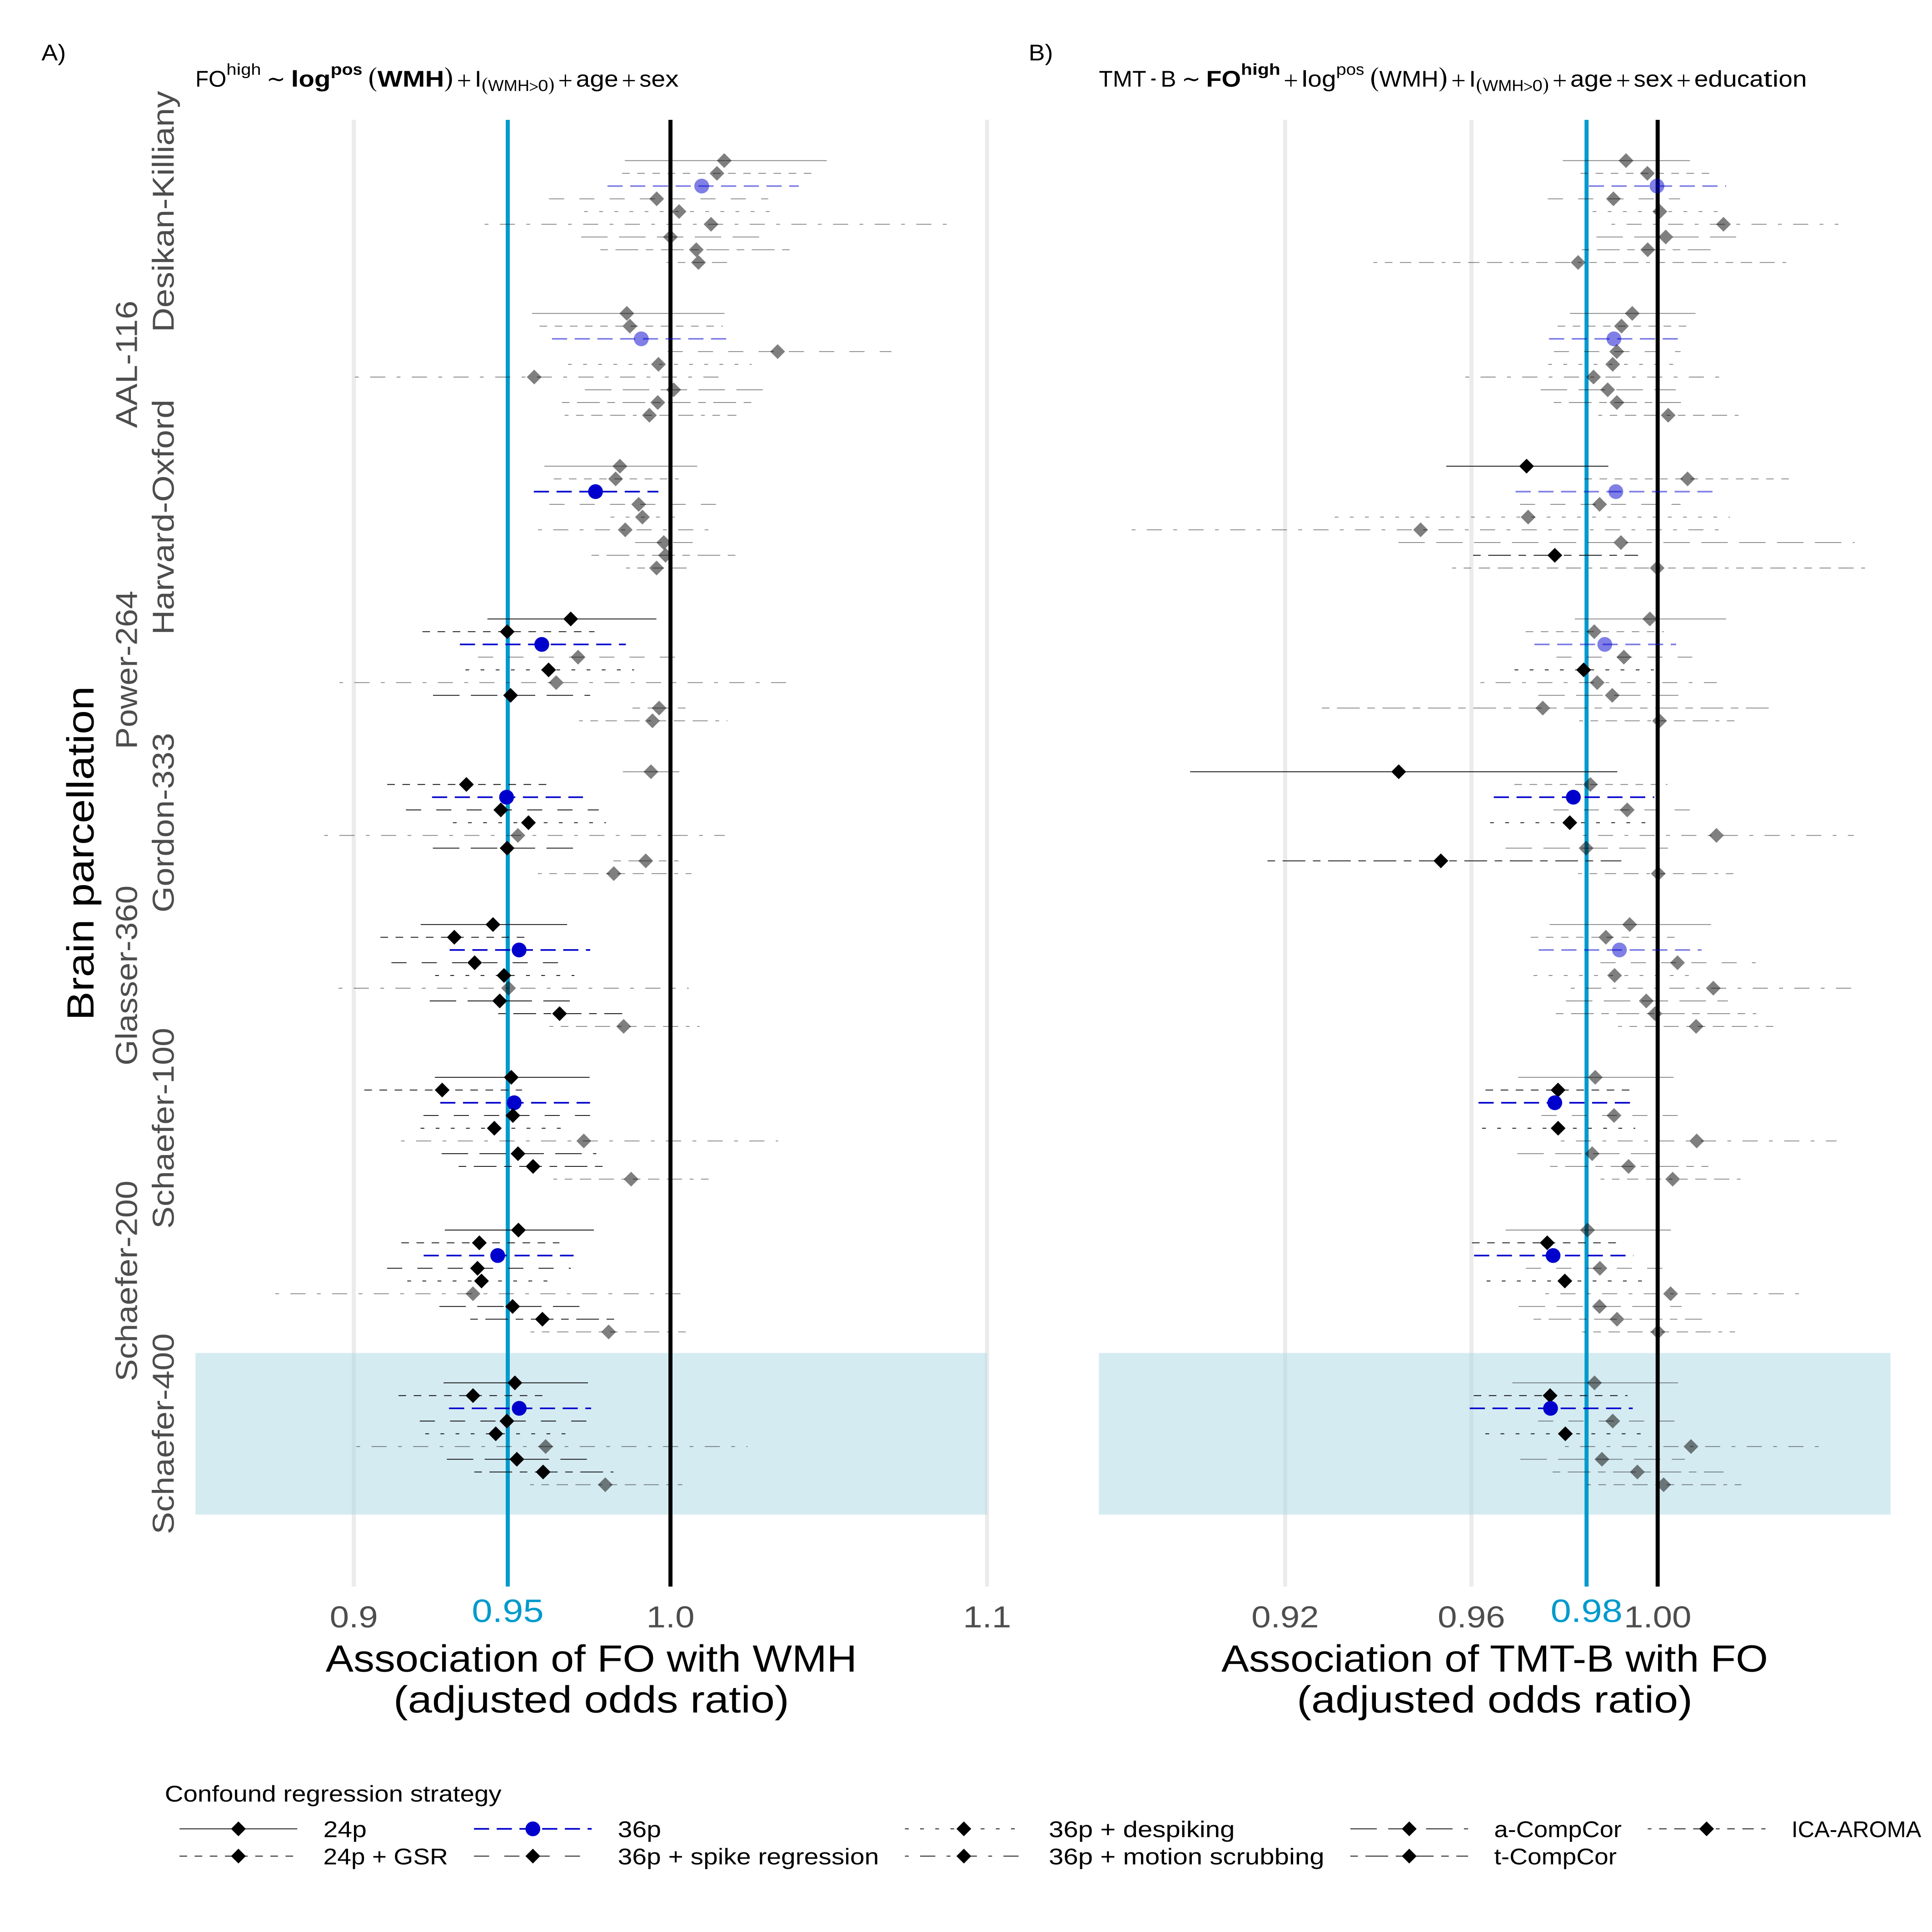
\includegraphics[width=\linewidth]{./../analysis/derivatives/Figures/Fig3deep.png}
    \captionof{figure}{\textbf{Multiverse analysis, deep WMH}}

    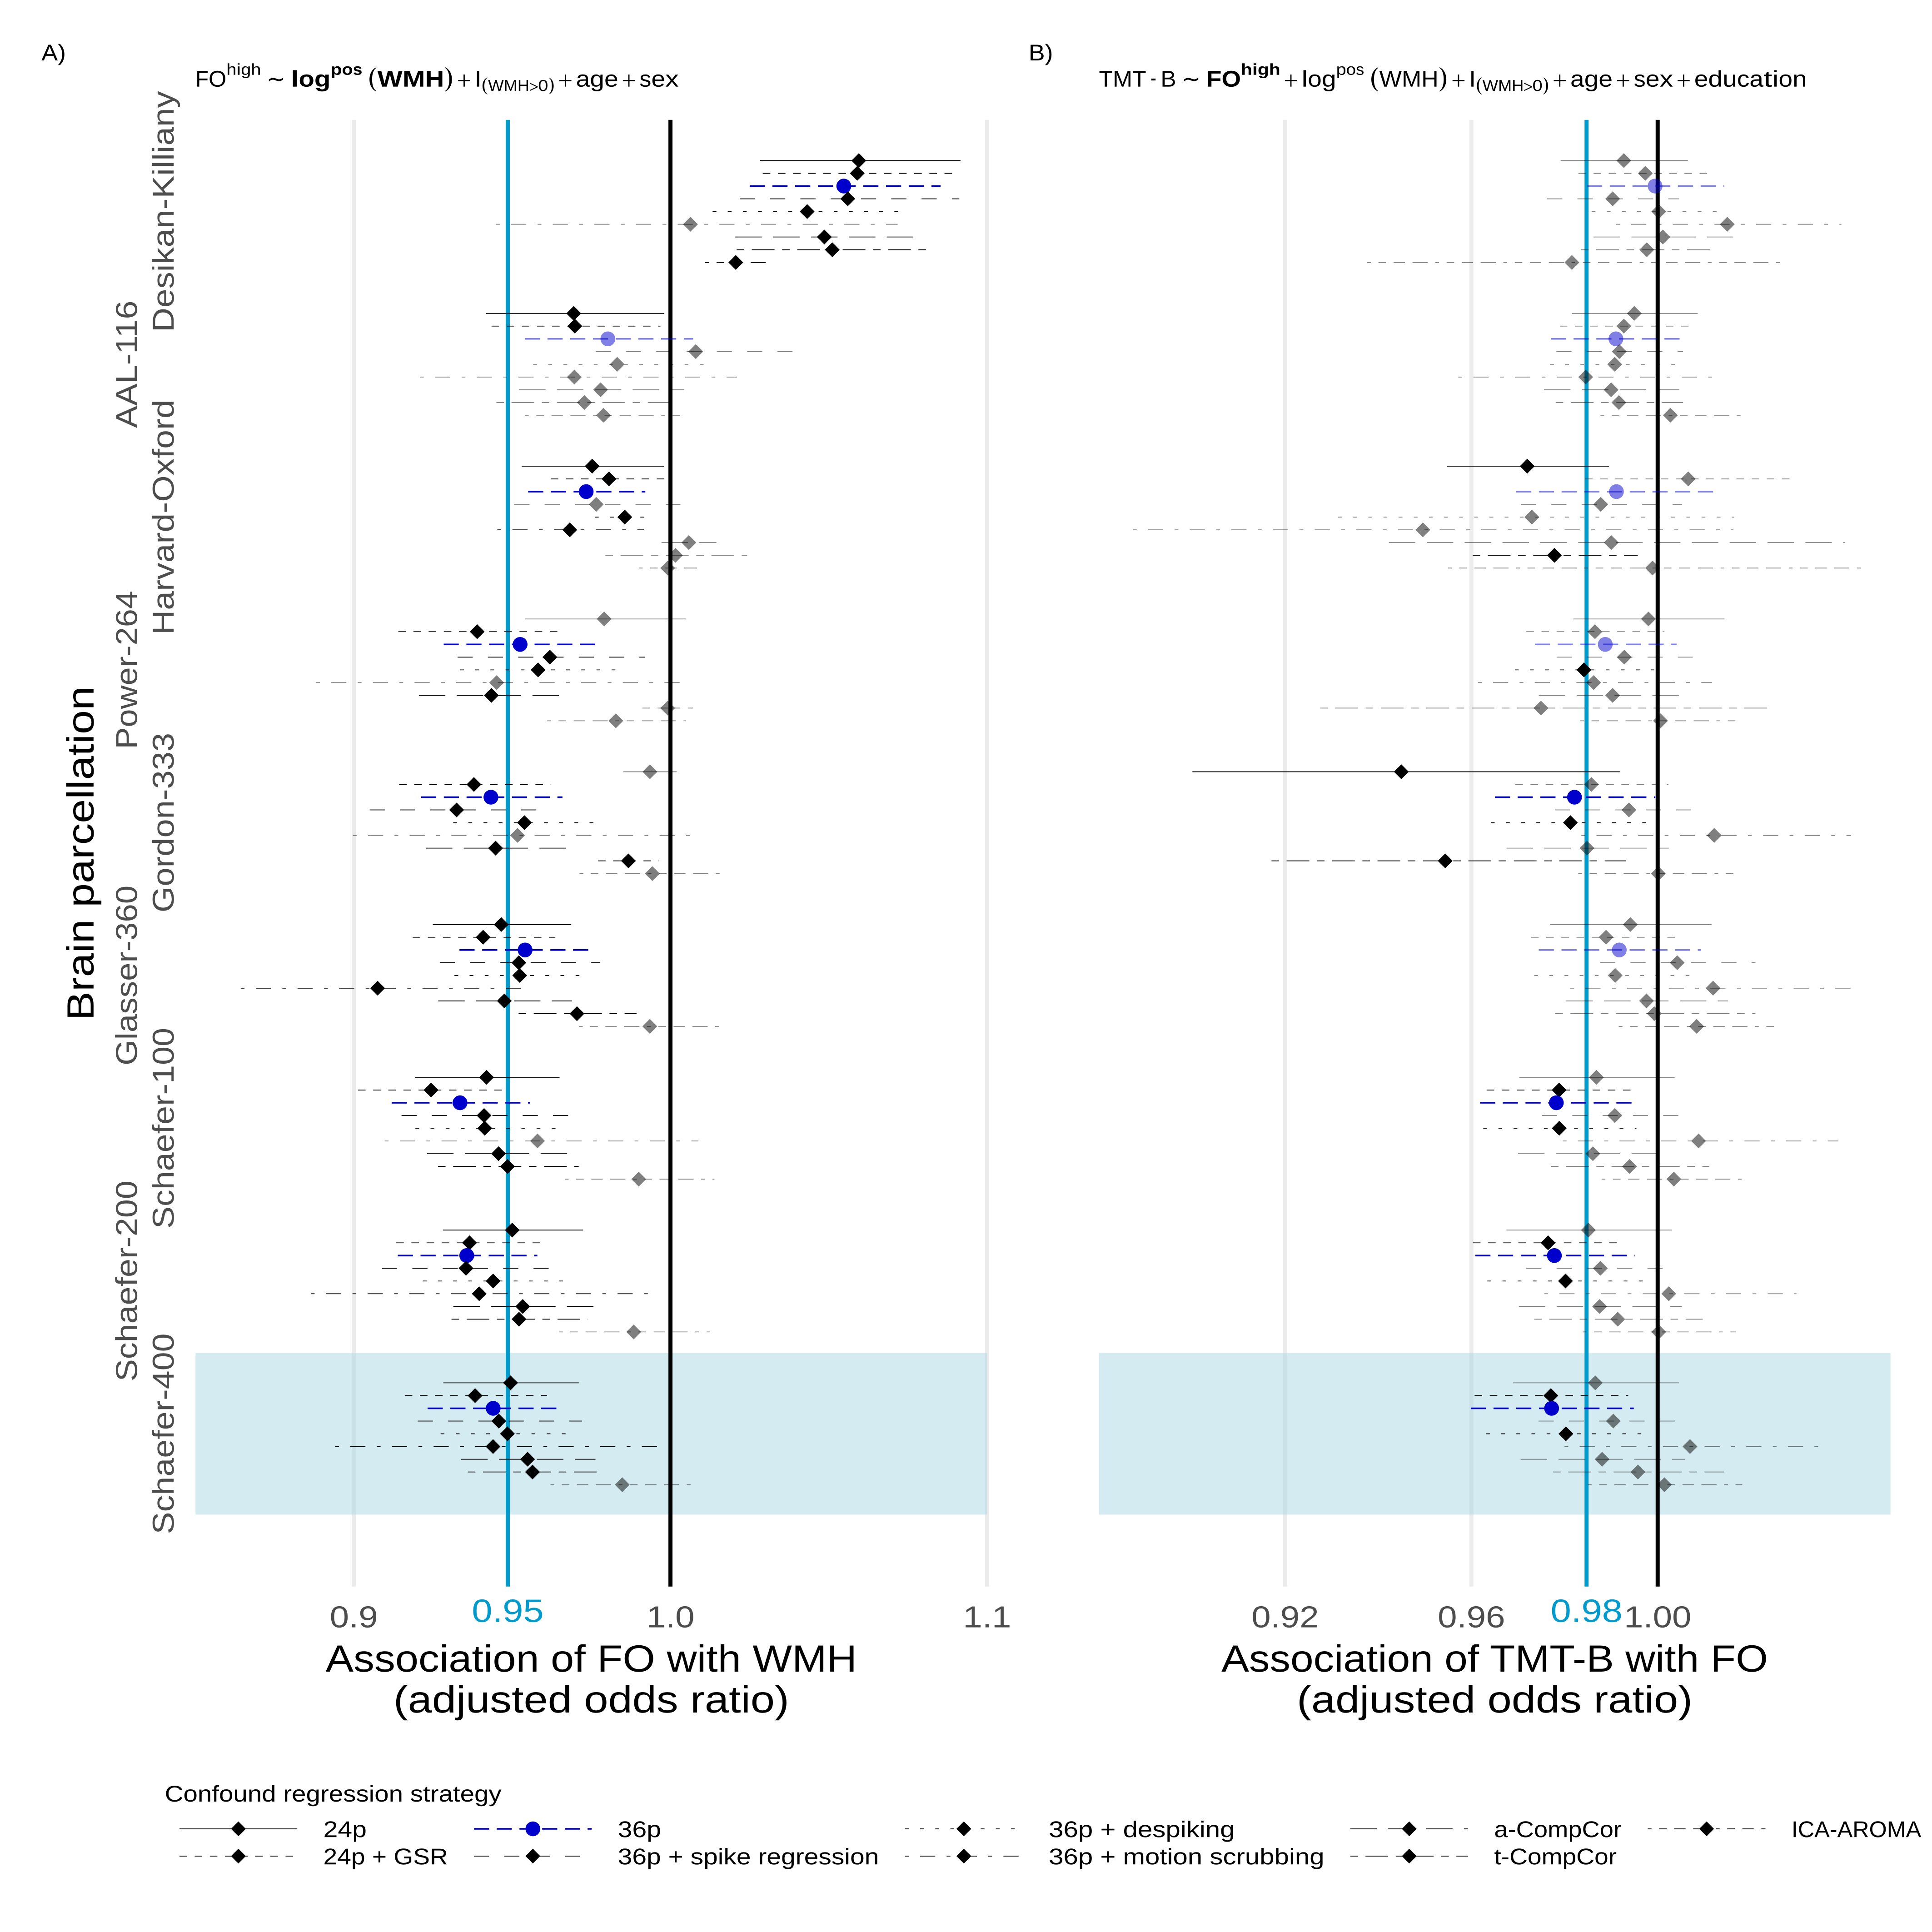
\includegraphics[width=\linewidth]{./../analysis/derivatives/Figures/Fig3peri.png}
    \captionof{figure}{\textbf{Multiverse analysis, periventricular WMH}}

\subsection{Motion parameters}
We also present, in analogy to \Cref{tab:hyp1,tab:hyp2}, regression tables for the association between time spent in DMN-related brain states (FO) and WMH volume, and between TMT-B and FO, adjusted for DVARS, RSMD and framewise displacement, in addition to age, sex and, in the latter case, years of education.

    \centering
    \setlength{\LTpost}{0mm}
    \begin{longtable}{lccc}
    \toprule
    & Estimate & P & 95\%-CI \\ 
    \midrule
    Intercept & 0.32 & <0.0001 & 0.28 -- 0.36 \\ 
    WMH, per 5.1-fold increase\textsuperscript{1} & 0.96 & 0.0004 & 0.94 -- 0.98 \\ 
    Age, per 10 years & 1.01 & <0.0001 & 1.00 -- 1.01 \\ 
    Female sex & 1.11 & <0.0001 & 1.08 -- 1.15 \\ 
    $\mathbf{1}_{\{\operatorname{WMH=0}\}}$ & 0.91 & 0.3552 & 0.74 -- 1.11 \\ 
    DVARS & 0.98 & <0.0001 & 0.98 -- 0.99 \\ 
    RMSD & 28.29 & 0.0055 & 2.67 -- 299.84 \\ 
    Framewise displacement & 0.16 & 0.0112 & 0.04 -- 0.66 \\ 
    \bottomrule
    \end{longtable}
    \textsuperscript{1} Interquartile ratio $2.37/0.468=5.06$
    \captionof{table}{Association between time-spent in high-occupancy DMN-related brain states and WMH volume adjusted for age, sex, and \textbf{motion parameters}}
    

    \centering
    \setlength{\LTpost}{0mm}
    \begin{longtable}{lccc}
    \toprule
    & Estimate & P & 95\%-CI \\ 
    \midrule
    Intercept & 46.83 & <0.0001 & 36.74 -- 59.72 \\ 
    $\operatorname{FO}^{\text{high}}$, per 5\%  & 0.71 & 0.0718 & 0.49 -- 1.03 \\ 
    WMH, per 5.1-fold increase\textsuperscript{1}  & 1.01 & 0.3414 & 0.98 -- 1.04 \\ 
    Age, per 10 years & 1.02 & <0.0001 & 1.01 -- 1.02 \\ 
    Female sex & 1.00 & 0.8171 & 0.96 -- 1.04 \\ 
    Education, per year  & 0.97 & <0.0001 & 0.97 -- 0.98 \\ 
    $\mathbf{1}_{\{\operatorname{WMH=0}\}}$ & 0.96 & 0.7581 & 0.73 -- 1.29 \\ 
    DVARS & 1.01 & 0.0001 & 1.00 -- 1.01 \\ 
    RMSD & 0.31 & 0.4695 & 0.01 -- 7.45 \\ 
    Framewise displacement & 1.08 & 0.9322 & 0.16 -- 7.13 \\ 
    \bottomrule
    \end{longtable}
    \textsuperscript{1} Interquartile ratio $2.37/0.468=5.06$
    \captionof{table}{Association between TMT-B and time spent in high-occupancy DMN-related brain states adjusted for age, sex, WMH volume and years of education, and \textbf{motion parameters}}